\documentclass{article}
\usepackage[utf8]{inputenc}
\usepackage{graphicx}

\title{TUGAS PEMROGRAMAN 2}
\author{DYAH AYU ANANDRA}
\date{17 Oktober 2019}

\begin{document}

\maketitle

\section{Sejarah Python}
\usepackage{Python merupakan bahasa pemrograman yang tingkatannya paling tinggi. Untuk membuat banyak program seperti, program CLI, program GUI (dekstop), Aplikasi Mobile, Web, IoT, Game dan lain-lain. Pemrograman Bahasa python merupakan pemrograman gratis atau freeware, sehingga dapat dikembangkan, dan tidak ada batasan tertentu dalam penyalinannya dan pendistribusiannya. Terdapat pelayanan yang disediakan lengkap dengan source codenya, debugger dan profiler, interface, fungsi system, Gui dan basisdatanya. Python tersedia untuk berbagai Sistem Operasi, Seperti Unix (Linux), PCs (DOS, Windows, OS/2), Machintosh dan sebagainnya.Python disempurnakan oleh Guido Van Rossum tahun 1990 di CWI, Amsterdam menjadi kelanjutan dari bahsa pemrograman ABC. Versi terakhir yang dikeluarkan oleh CWI adalah 1.2. Tahun 1995, Guido berpindah ke CNRI dengan terus mengembangkan Python. Versi terakhir yang dikeluarkan adalah 1.6. tahun 2000, Guido dan pengembang inti Python berpindah ke BeOpen.com yang melahirkan sebuah perusahaan komersial dan membentuk BeOpen PythonLabs.}

\section{Perbedaan Python 2 dan Python 3}
\subsection{Python 2}
\usepackage{Python versi 2.0 dikeluarkan oleh BeOpen. Setelah mengeluarkan Python versi 2.0, Guido dan anggota tim PythonLabs pindah ke DigitalCreations. Saat ini pengembangan Python terus saja dilakukan oleh para sekumpulan pemrogram yang dikoordinir oleh Guido dan Python Perangkat Lunak Foundation. Python Perangkat Lunak Foundation merupakan lembaga  non-profit dibentuk sebagai pemegang hak cipta dari intelektual Python mulai dari versi 2.1 demikianlah mencegah Python dimiliki oleh perusahaan komersial. Saat ini pendistribusian Python telah mencapai versi 2.6.1. Python Versi 2  merupakan versi yang banyak sekali digunakan saat ini, seperti dilingkungan produksi dan pengembangan. Untuk membuka python versi 2 hanya dengan menggunkan perintah python saja.}

\subsection{Python 3}
\usepackage{Python versi 3.0. Nama Python dipilih oleh Guido sebagai nama bahasa ciptaannya karena kecintaan guido pada sebuah acara televisi Monty Python's Flying Circus. Oleh karena itu seringkali ungkapan-ungkapan khas dari acara tersebut sering muncul dalam korespondensi antar pengguna Python. Python Versi 3 merupakan perkembangan dari Python versi 2 dan lebih banyak memiliki fitur terbaru dibandingkan Python 2. Untuk membuka Python versi 3 menggunkan perintah Python3.}

\section{Implementasi dan Penggunaan Python di Perusahaan Dunia}
\usepackage{Seperti yang sudah diketahui, Python telah banyak digunakan oleh lingkungan akademis dan startup karena Python sederhana. Namun, seringkali solusi sederhana adalah yang paling terbaik. Semakin kompleks aplikasi, maka semakin terbuka kemungkinan untuk melakukan kesalahan, banyak perusahaan besar yang tidak mau dengan kesalahan karena akan menrusak reputasi mereka, karenanyalah kenapa banyak perusahaan dan aplikasi besar menggunakan Python, dengan tools yang sederhana, terbukti dapat melahirkan aplikasi yang sangat mengagumkan. Berikut beberapa perusahaan dunia yang menggunakan Python.}
\begin{enumerate}
    \item Google Dari awal berdiri, Google sudah menggunakan Python, bahkan Python adalah salah satu bahasa pemrograman yang penting bagi Google.
    \item Industrial Light and Magic Menggunakan Python, ILM dapat dengan mudah mengemas komponen software dan meningkatkan aplikasi grafis mereka.
    \item Netflix merupakan Aplikasi RESTful ini akan me-reroute alert dan mengirimkannya ke kelompok atau individu yang berhak melihatnya. 
    \item Instagram Seperti yang kita ketahui, Instagram telah merevolusi komunikasi visual dan pemasaran digital melalui media foto.
    \end{enumerate}
\usepackage{Selain perusahaan yang ada diatas, ada beberapa perusahaan lain yang menggunakan Python.}
\begin{enumerate}
    \item Pinterest
    \item Disqus
    \item Dropbox
    \item Uber
    \item Reddit
    \item Quora
    \item Facebook (Bahasa ke-3 setelah PHP (Hack) dan C++, digunakan untuk manajemen infrastruktur)
    \end{enumerate}
    
\section{Instalasi Anaconda}
\begin{enumerate}
    \item Pertama download terlebih dahulu file anaconda
    \item Buka setup anaconda untuk memulai instalasi
    \item Ketika layar seperti dibawah sudah muncul, maka klik next
    \graphicspath{width}
    \begin{center}
        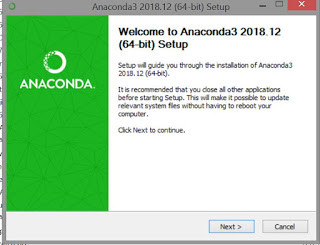
\includegraphics[width = 10cm\textwidth]{cara1.JPG}
    \end{center}
   
    \item Kemudian baca lisensi perjanjian terlebih dahulu, lalu klik I Agree
    \begin{center}
        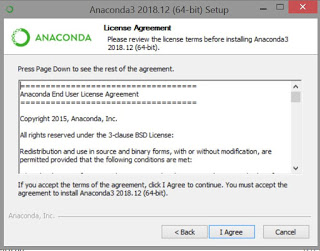
\includegraphics[width = 10cm\textwidth]{cara2.JPG}
    \end{center}
    \item Pilih just me, lalu klik next
    \begin{center}
        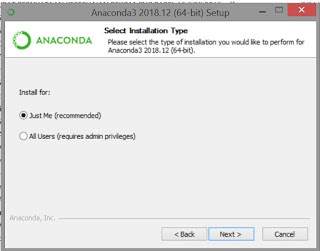
\includegraphics[width = 10cm\textwidth]{cara3.JPG}
    \end{center}
    \item Tentukan folder untuk menyimpan dimana
    \begin{center}
        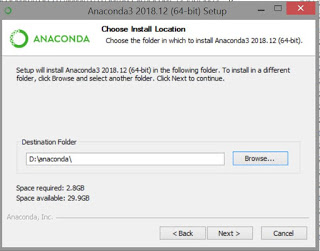
\includegraphics[width = 10cm\textwidth]{cara4.JPG}
    \end{center}
    \item Di opsi pasang lanjutan ceklist atas dan bawahnya, lalu klik install
    \begin{center}
        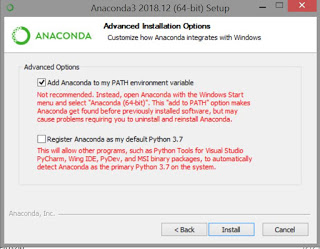
\includegraphics[width = 10cm\textwidth]{cara5.JPG}
    \end{center}
    \item Klik finish
    \begin{center}
        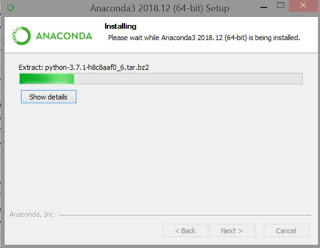
\includegraphics[width = 10cm\textwidth]{cara6.JPG}
    \end{center}
    \item Tampilan navigator 
    \begin{center}
        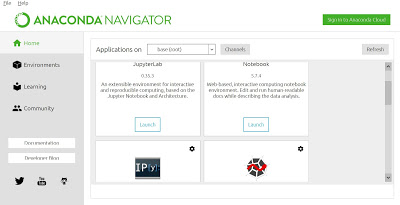
\includegraphics[width = 10cm\textwidth]{cara7.JPG}
    \end{center}
    \end{enumerate}
    
\section{Intall pip}
\usepackage{Ketikan pip di cmd, jika tidak ada masalah, maka paket akan terinstal dengan sukses dan bisa kita pakai untuk membuat program. jika belum sukses, pip akan menampilkan pesan error yang menunjukkan di mana letak kesalahannya.}
\section{Cara Setting Environment}
\begin{enumerate}
    \item Masuk ke system pada Control Panel Control Panel and Security
    \item Kemudian klik Advanced system settings\\
    \graphicspath{width}
    \begin{center}
        \includegraphics[width = 10cm\textwidth]{}
    \end{center}
    \item Lalu klik Environment Variable maka akan muncul lagi Environment Variable
    \item Pada bagian System variables, scroll sampai ketemu Path. (Path adalah nama Variable)
    \graphicspath{width}
    \begin{center}
        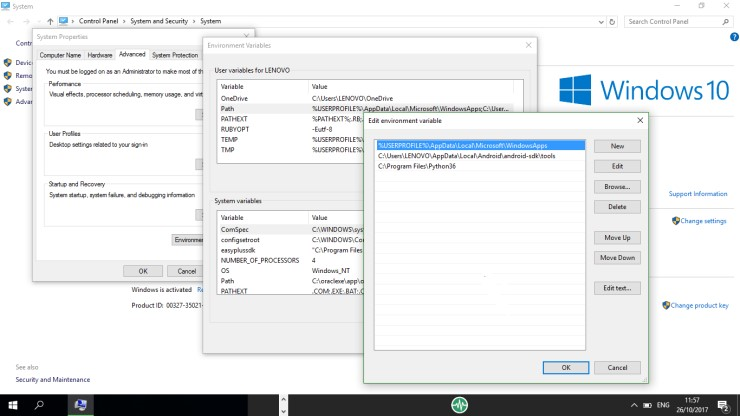
\includegraphics[width = 10cm\textwidth]{set2.jpg}
    \end{center}
    \item klik Path dan kemudian klik Edit
    \item Maka akan muncul lagi Edit System variable
    sebelum mengedit Variable value buat terlebih dahulu backup untuk mencegah  hal-hal yang diluar dugaan, buka notepad copas semua Variable value
    \item Pada bagian paling kanan/ujung Variable value
    tambahkan path ;C:\Python\  tanpa tanda petik
    dan klik OK pada jendela Edit System variable
    \item klik OK pada jendela Environment Variables.
    klik OK pada jendela System Properties
    dan close Control Panel
    \end{enumerate}
    
\section{mencoba entrepreter/cli melalui terminal atau cmd windows}
\begin{enumerate}
    \item Buka cmd, ketik python
    \item Ketik perintah di cmd
    \end{enumerate}
    
\section{Cara Menjalankan Script hello world di spyder}
\begin{enumerate}
    \item Buka spydernya terlebih dahulu
    \item lalu tiliskan perintah
    \begin{center}
        \includegraphics[width = 10cm\textwidth]{helo.jpg}
    \end{center}
    \item setelah itu kita run
    \item menunggu hasil
    \end{enumerate}
    
\section{variable Explorer}
\usepackage{Explorer Variabel memperlihatkan konten  yang semua referensi objek global, seperti variabel, fungsi, modul, dll. Dari sesi Konsol Python yang saat ini dipilih, dan memungkinkan Anda untuk berkolerasi dengan mereka melalui editor berbasis GUI. Variable Explorer mempunyai editor khusus untuk serangkaian objek Python internal dan pihak ketiga umum, dan dapat melihat, mengedit, dan mengintrospeksi objek paling sewenang-wenang melalui objek Penjelajah objek yang lebih umum. Jenis dengan dukungan pengeditan khusus meliputi:}
\begin{enumerate}
    \item Integer
    \item Mengapung
    \item Bilangan kompleks
    \item String
    \item tanggal datetime dan Timedelta s
    \item Daftar
    \item Tuples
    \item Kamus
    \item Array dan matriks NumPy
    \item DataFrame Pandas, TimeSeries dan DatetimeIndex
    \item PIL/Pillow
    \item Ruang nama
    \end{enumerate}

\section{Identasi}
\subsection{Penjelasan Identasi}
\usepackage{Di dalam Bahasa pemrograman Python manfaat identasi adalah sebagai menutup atau membuka suatu fungsi.}

\subsection{Jenis-Jenis Error Identasi Yang Didapat}
\begin{center}
        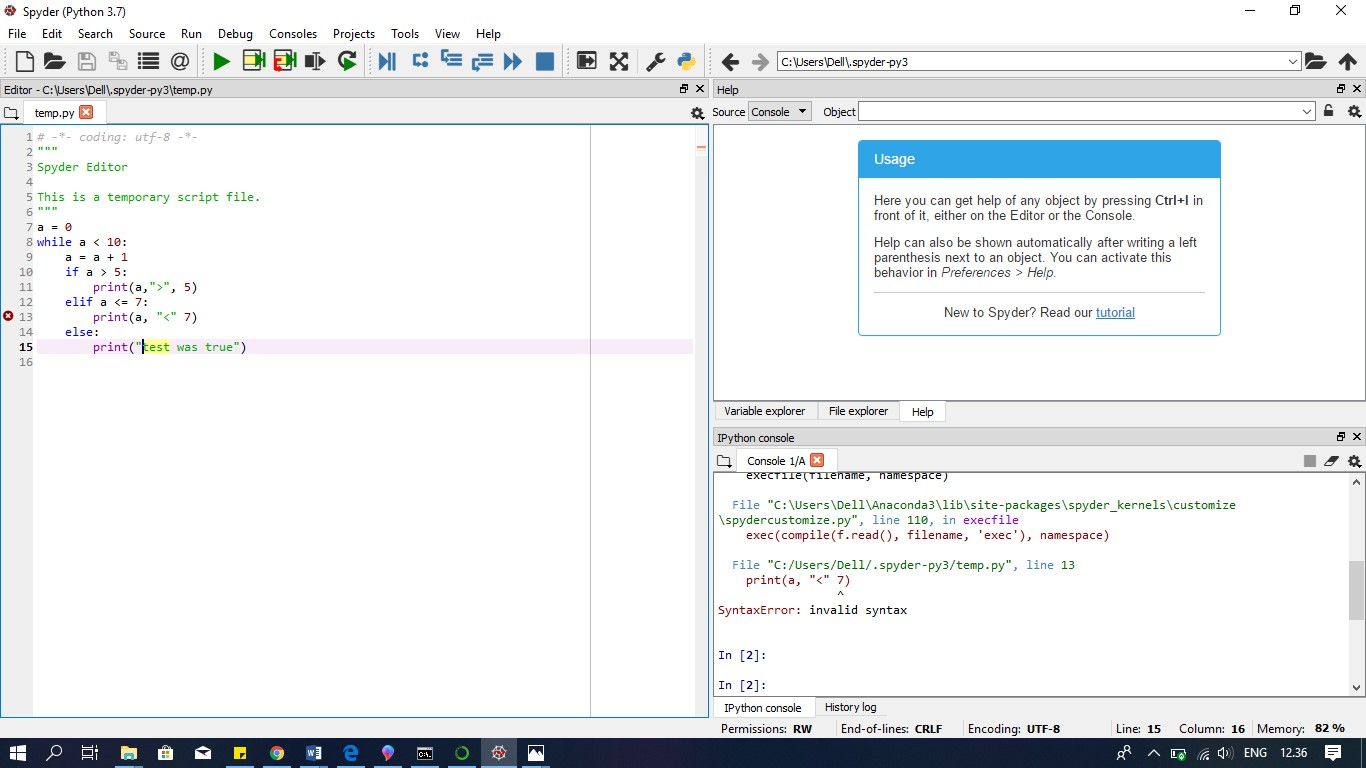
\includegraphics[width = 10cm\textwidth]{tax.jpg}
    \end{center}
    
\usepackage{Keadaan error sering kita jumpai di dalam suatu syntax oleh sebab itu diperlukan adanya ketelitian dalam penulisan seperti penulisan tanda baca, type data, dan lain-lain. cara menangani errornya perlu adanya perbaikan, dicek ulang dengan teliti.}

\end{document}
